% 5TH WORKSHOP C4EU

\documentclass[a4paper,twocolumn]{IEEEtran}
\usepackage[utf8]{inputenc}
\usepackage{graphicx}

\title{
    Open Sensor Network\\
    Platform improvement
}

\author{
    Alejandro Andreu Isábal\\
    \texttt{alejandro.andreu01@estudiant.upf.edu}
}

% BEGIN DOCUMENT
\begin{document}

    % Make title
    \maketitle

    % -Arduino
    \section{Usage of XBee Direct I/O}

    The initial version of the project used the well-known prototyping platform Arduino, which allowed to send data with a small amount of LOC (lines of code) below an XBee module.

    XBee's have two operation modes, AT and API modes, each one explained below:
    \begin{description}
        \item[AT] Also called \emph{transparent mode}, which is simple and allows communication with any device that ``speaks'' \emph{serial}. However, it has limited point-to-point capabilities with other XBee devices.
        \item[API] Although it is more complex, it allows to exploit the full potential that an XBee has. That is, using all the pins available and configuring them separately to do things.
    \end{description}

    Some of the pins mentioned above can be set in many modes, including analogic input, digital input and digital output. This, together with a sampling rate can lead to a project where no Arduino is necessary, since the XBee does all the work itself.

    This has many advantages including less power consumption, much cheaper design. However, this increases the overall difficulty of the project, because it requires electronic knowledge, and also some library re-implementation could be necessary.

    But without a doubt, the most useful feature that API mode brings with itself is that it encapsulates all the information in one well-structured packet.


    \section{Server-side script}
        
    Since an XBee must be attached to the server we need some kind of program to handle all this data. In order to reuse some bits of code and because of its simplicity and flexibility a \emph{Python 2.7.x} script is used again.

    The code has been significantly polished and its more sofisticated than in the previous version. The program now accepts arguments including \texttt{-h} or \texttt{--help} to see the flags that can be set as well as mandatory arguments.

    It works as an \emph{asynchronous} dispatcher, since it can receive many packets and spawn a new thread for each one of them. Thus a general overview of the program can be depicted as follows:

    \begin{center}
        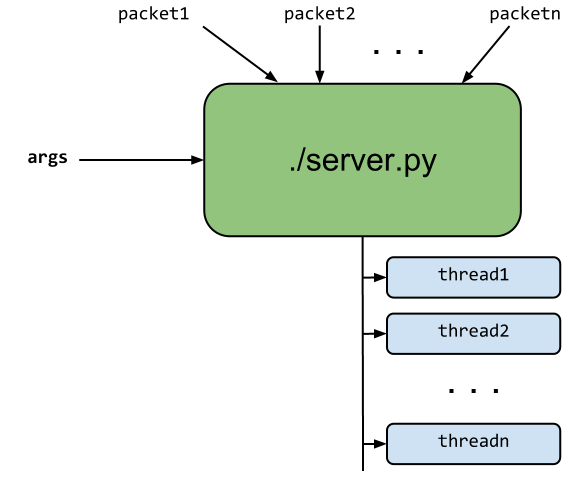
\includegraphics[scale=0.35]{server.png}
    \end{center}

    Each thread then serializes the data and writes a \emph{JSON} in order to upload the information to \emph{Cosm} through a shell script.


    \section{Future work}

    In order to see what the energy consumption what might actually be like, there shall be some testing with a lithium battery and a solar panel, which could be used at the same time as a solar radiation sensor.

    Also, to reduce consumption as well the XBee's can be in \emph{sleep mode}, wich wakes up the device every now and then and transmits a packet.

\end{document}
